\section{Aufbau}
\label{sec:Aufbau}

Für den Versuch wird ein Aufbau wie in Abbildung \ref{fig:aufbau} benutzt.
\begin{figure}
  \centering
  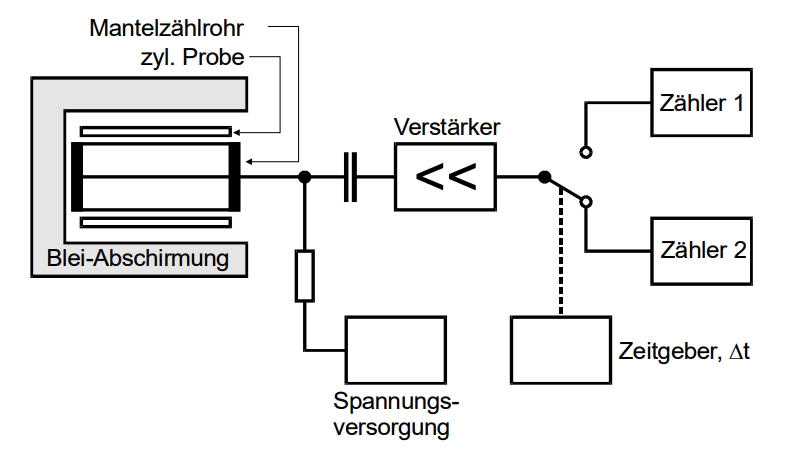
\includegraphics[height=6cm]{data/Aufbau.png}
  \caption{Skizze des Versuchaufbaus.}
  \label{fig:aufbau}
\end{figure}
Ein Geiger-Müller-Zählrohr registriert einen konstanten Anteil der Strahlung der radioaktiven Probe.
Beide Komponenten befinden sich innerhalb einer Blei-Abschirmung, um den Einfluss der natürlichen Radioaktivität (Nulleffekt) zu minimieren.
Der im Zählrohr durch ein radioaktives Teilchen ausgelöste Ladungsimpuls wird verstärkt und von einem der Zähler aufgezeichnet.
So werden die Zerfälle, die in einem Zeitintervall $\increment t$ aufterten, abwechselnd von einem der beiden Zähler ermittelt.
Das Zeitintervall $\increment t$ kann beliebig eingestellt werden.
